\section{EXPERIMENT 2: RECOGNITION OF THE FRICTION FIELD LOCATION}

%Unlike the previous experiment where the resultant force vector of all pins was the same, 
In this experiment, the recognition of force distribution was investigated.
We assumed a field in which the friction coefficient varies in a distributed manner.
The distribution follows the cosine function and is largest at the center and smaller with distance from the center.
Participants were asked to find the center of the frictional field on the virtual surface.
Participants wore the device and explored the surface and found the position by resorting to frictional force distribution provided by the device.

The number of participants was five (four males and one female, aged between 23 to 26).

\subsection{Experimental Environment}

In this experiment, only the 60$^{\circ}$ device was used. 
This is because the 60$^{\circ}$ device has the smaller JND than the 45$^{\circ}$ device.
As in Experiment 1, participants sat on a chair and explore the surface with the device. 
The position of their finger was measured using a magnetic sensor and it was sent to the simulation. 
During exploration, participants could see the display the position of the virtual finger on the virtual surface on display. Blue nodes corresponded to the pair of pins (Fig.\ref{fig_experimental_window}).

% We recorded the center coordinates of the participant finger. 

\begin{figure}[h]
  \centering
  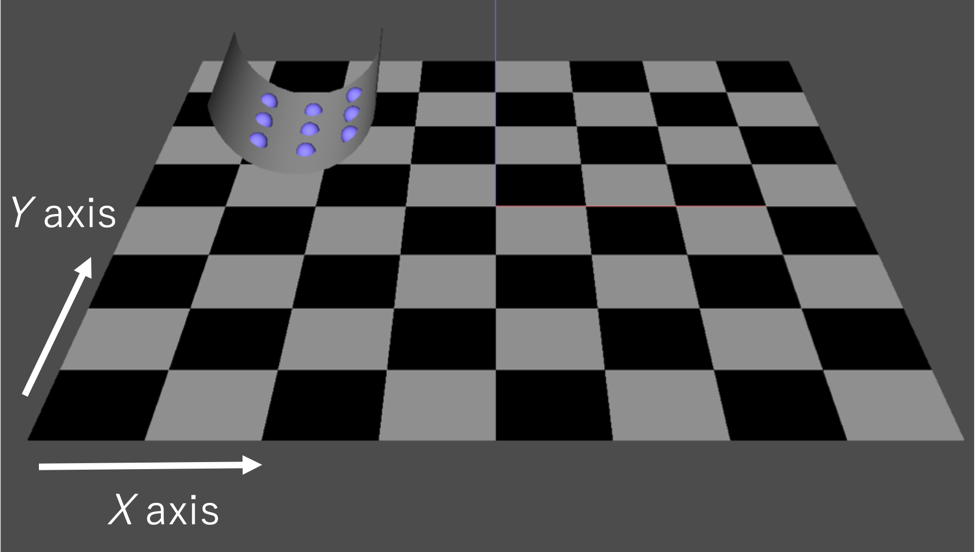
\includegraphics[width=2.9in]{images/fig_experimental_window.png}
  \caption{Participants watched the position of virtual finger on virtual surface. Blue nodes corresponded to the pair of pins}
  \label{fig_experimental_window}
\end{figure}

We designed a "friction field" in which friction coefficient varies in a distributed manner with a radius of 20 mm on the virtual surface with 80mm $\times$ 80mm.
Nine center coordinates of the friction field visualized in black in Fig.\ref{fig_friction_position} were prepared. 
One of them is visualized in red in Fig.\ref{fig_friction_position}. 

\begin{figure}[h]
  \centering
  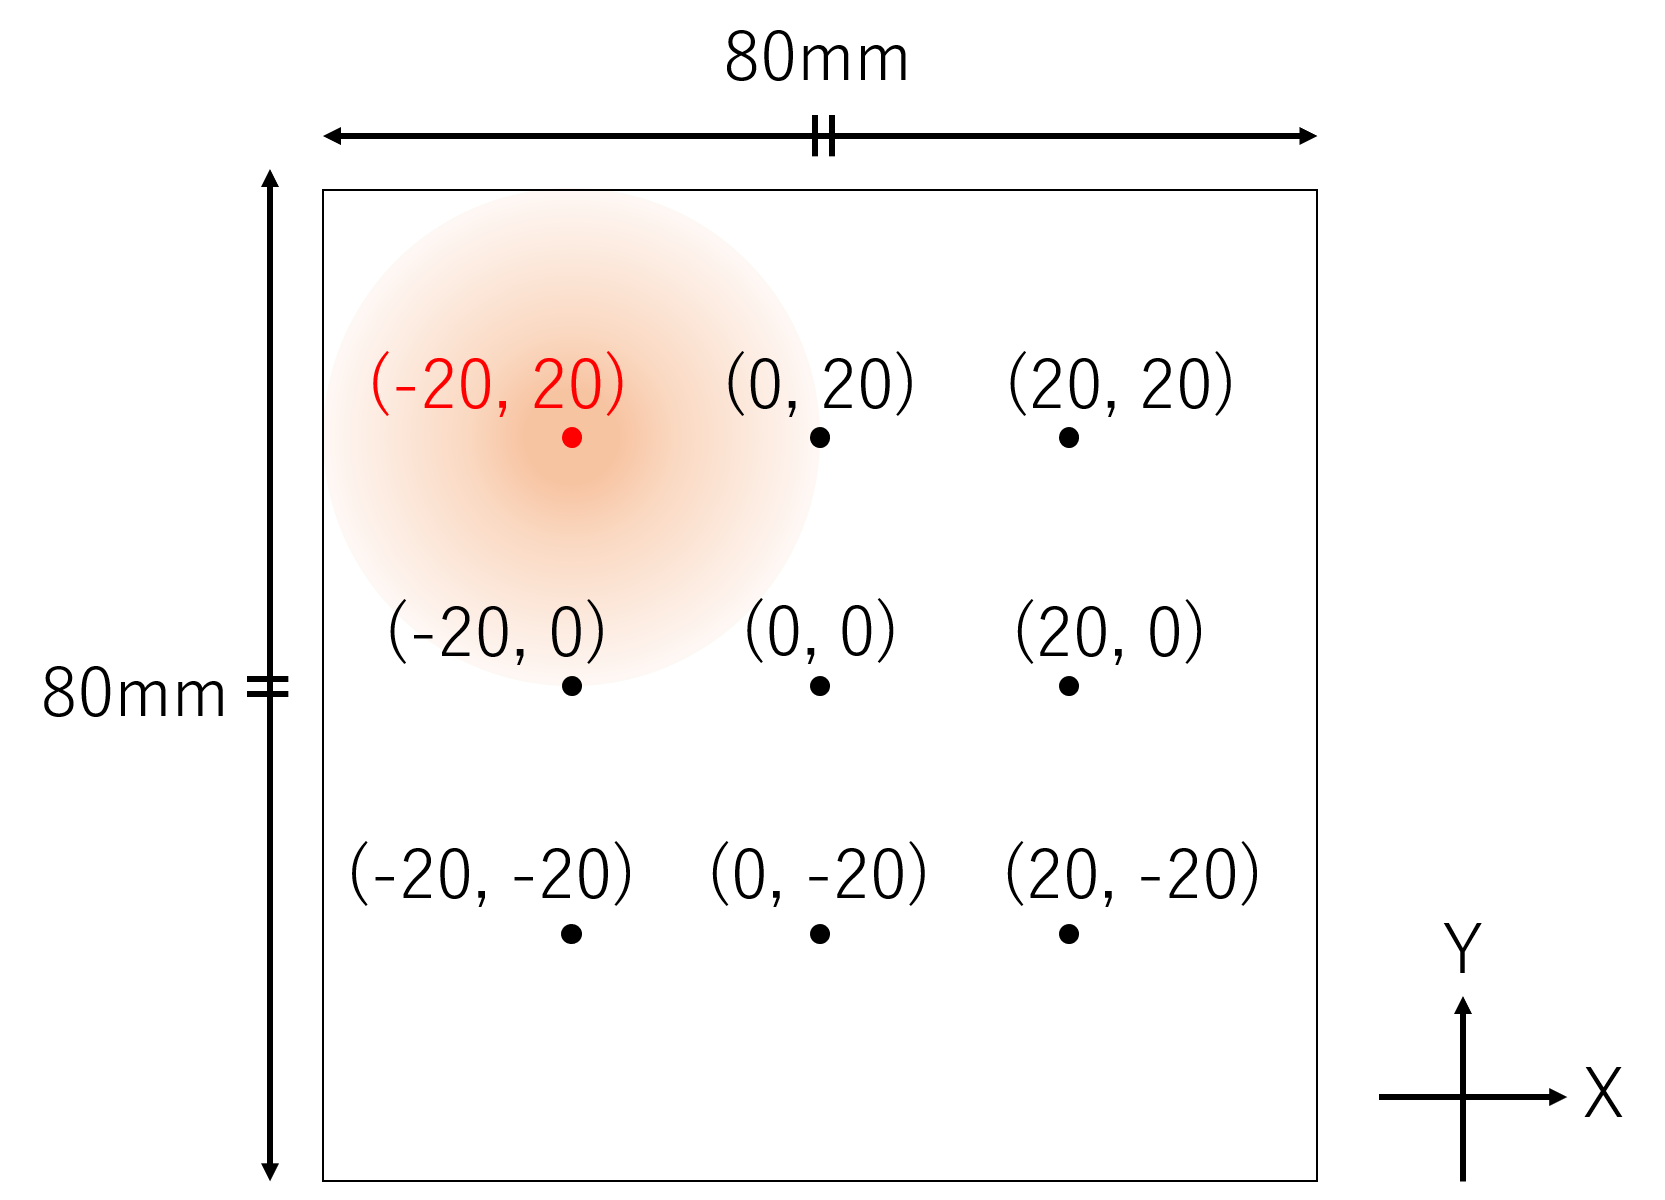
\includegraphics[width=2.1in]{images/fig_friction_field}
  \caption{Nine candidate of center coordinate of friction field. One of the friction field is visualized.}
  \label{fig_friction_position}
\end{figure}

% The friction coefficient of the friction field varied depending on the distance from the center.
The friction coefficient was 1 at the center and its value decreased from the center towards the outside. 
It was determined by the following formula:

\begin{equation}
    \mu = (\cos{\frac{\pi r}{2 radius}})^2
\end{equation}

where $\mu$ is the friction coefficient at that coordinate. 
$r$ is the distance from the center of the friction field (mm), and $radius$  is the radius of the friction field (20 mm).
$\mu$ defined the resultant force ($F_{X}$, $F_{Z}$) as follows:

\begin{equation}
\label{F_z}
    F_{Z} = k \cdot \Delta z 
\end{equation}
\begin{equation}
\label{F_x}
    F_{X} = - \mu \cdot \mathrm{sgn}(v) \cdot k \cdot \Delta z
\end{equation}

where $v$  is the direction component of the finger obtained by dividing the velocity vector by the absolute velocity value, $k$ is the elastic modulus (0.1), and $\Delta z$ is the distance penetrated by the finger into the virtual surface (mm). 
The force output to each pin $F_{R}$, $F_{L}$ of the device is determined by expression (\ref{F_x})(\ref{F_z}), and (\ref{eq:2}).

\subsection{Task Design}

The experiment consisted of a practice phase and an evaluation phase. 

In the practice phase, participants could feel the frictional cue in order to familiarize themselves with the operation of the device only once.
After that, the evaluation phase was carried out.
In the evaluation phase, participants were instructed to find the center of the friction field.
Participants could freely move their index finger with the device on the surface without a time limit.
When they found the center, they put their thumb on it and pushed the button of the keyboard.
Participants were instructed to search with the thumb orientation fixed in the $Y$ axis direction.
% Also, Participants explored while looking at the positional relationship between their fingertip and the floor (Fig. 9 (a)).  % ちょっとよくわからなかった..

The trials of exploration were conducted 36 times, nine center coordinates of the friction field were prepared and randomly determined.

\subsection{Data Analysis}

We preprocessed the obtained data to compensate individual differences of the center coordinate of their fingertips.
We assume that the mean value of the responses for each participant was the center coordinates of the participant’s fingertips.
Thus, we obtained the compensated value by subtracting the value from each answer value for each participant. 
We performed a single round of 3$\sigma$ clipping to remove
outliers. 
The following analysis was performed on the data that did not include outliers.

With this device, with regard to the $X$ axis, participants received frictional cues as shear and normal force distribution expressed in equation (\ref{F_x}) and (\ref{F_z}) respectively.
%In contrast, with regard to the $Y$ axis, participants only received normal force distribution in expression (\ref{F_z}).
While, with regard to the $Y$ axis, no tangential component caused by the friction was presented.
To determine whether there is a difference in error along $X$ and error along $Y$ axes, we conducted the t-test per participant.

\subsection{Result}

\begin{figure}[h]
  \centering
  \includegraphics[width=3.0in]{images/fig_ex2_res}
  \caption{Recorded fingertip coordinates of each participant (mm).}
  \label{fig_ex2_res}
\end{figure}

\begin{table}[h]
  \centering
  \caption{Standard deviation of each participant (mm).}  
  
\includegraphics[width=3.2in]{images/tbl_ex2_res}
  \label{tbl_ex2_res}
\end{table}

We removed three outlier samples that were out of a 3$\sigma$ range.
All of the removed samples were the ones obtained from participant No.2.
We plot the compensated value of each participant when the center of friction field was (0,0) in Fig.\ref{fig_ex2_res}.
% In all participants except the participant 2, the center coordinates of the fingertip were located in a friction field with a radius of 20 mm in all trial. 

% The center coordinate of the fingertip varies depending on individual differences, time, and circumstances.
% In order to correct these differences, the mean value of the responses of each participant was taken as the center coordinates of the participant's fingertip, and a value obtained by subtracting the coordinates of the participant's fingertip from each answer value of the participant was taken as the compensated value.

Table.\ref{tbl_ex2_res} shows the standard deviation of along $X$ and $Y$ axes for each participant. 
%According to the t-test, there is a significant difference in standard deviation between $X$ and $Y$ axes for only participant No.2 ($p<0.01$).
According to the t-test result in standard deviation between $X$ and $Y$ axes, there was no significant difference other than No.2 ($p<0.01$).

\subsection{Discussion}

The results show that participants accurately recognized the position of the friction field (Fig.\ref{fig_ex2_res}).
And, the standard deviation represents the error of the participant fingertip's $X$ and $Y$ coordinates from the center of the friction field.
The error between true center position and the answered position were varied from participant to participant (Table.\ref{tbl_ex2_res}).

According to the t-test result, the difference in error along $X$ and $Y$ axes are significant for participant No.2.
This suggested the effect of shear force distribution feedback to users.
The participants were able to determine the center based on the distribution of shear force feedback by moving his finger in the X-axis direction.

%指をx軸方向に揺さぶりながらy軸方向に進めることで,y軸方向の摩擦分布を理解可能
%x, y軸の標準偏差に差が見られなかった原因かも
In contrast, there were no significant differences for other participants'{} data.
One of the reason of the result is that participants were able to recognize the center along the $ Y $ axis with the help of the $ X $ axis shear force feedback.
First, participants recognized the intensity of the local friction at a certain point by shaking their finger along the $X$ axis.
Then, participants moved their finger along $Y$ axis and compared the intensity of local friction along $Y$ axis.

% In this experiment, it was possible to understand the friction distribution in the $Y$ axis direction by moving the finger in the $Y$ axis direction while shaking the finger in the $X$ axis direction.
% Therefore, it is considered that there was no significant difference in the standard deviation between the $X$ axis and the $Y$ axis direction.

%One of the reason why there was no significant difference is that the task was easy and thus, normal indentation was enough to recognize the center position.

We are considering two plans as future work. 
The first plan is to make the contact point denser by miniaturization of the pins.
The second plan is to increase the degree of freedom that the device can present the stimulus. 
Currently, this device is possible to present the 2-DoF direction of the finger. In addition to this, we plan to add one more DoF by increasing the number of pins of 1 pair to 3, aiming at interaction with more natural objects.



% Considering that the distance between the pins of the device is 3.0 mm, the standard deviation of participants No.1, No.3 and No.4 were close to the distance between the pins.
% This indicates the possibility that participants 1, 3 and 4 were able to recognize the change in force output from the pair pins that tilted to the right and the left arranged at $3 \times 3$. 
% However, it has been confirmed that the stimulus shift discrimination threshold is 10 to 30 times smaller than the 2-point discrimination threshold when the stimuli shifts [9]. 
% Considering that the 2-point discrimination threshold of the human fingertip is 2mm to 3mm [15], it can be seen that there is a large gap between the variation from the center of the friction field obtained in this experiment and the stimulus shift discrimination threshold. 
% In addition, there is a mismatch in the action point of the left and right stimulus of this device, so that there is a possibility that the sense of discomfort might disturb the recognition of the subject. 